Vehicular Ad-hoc Networks (VANET) is one type of Mobile Ad-hoc Networks (MANET) that specially designed for moving cars. Three types of VANET applications are provided: 

Road safety applications including warning applications and emergency vehicle warning applications is the most valuable application of VANET. The safety application messages have the top priority among other communication services. The second type of application is Traffic management applications, which provides local and map information in order to improve traffic efficiency. The last type of application is for infotainment, which is based on the traditional IPv6 based internet. 

VANET supports two types of communications: Vehicle to Vehicle (V2V) communication: in VANET, each vehicle will be equipped with an On Board Unit (OBU). V2V communication is between the OBUs of each vehicle mainly for road safety applications and traffic management applications. 

Another type of VANET communication is Vehicle to Infrastructure (V2I). In VANET, the roadside infrastructure may be equipped with a RoadSide Unit (RSU). The V2I communication is between the RSU and the OBU mainly for infotainment applications. 

VANET is based on several protocols. Basically saying, the physical and MAC layers are defined in IEEE 802.11p. The above layers are defined in IEEE 1609.x protocols, also known as Wireless Access in Vehicular Environment (WAVE) stack. The PHY layer is defined in IEEE 802.11p, which currently has been cooperated with IEEE 802.11-2012. 

\begin{figure}[h!]
	\centering
	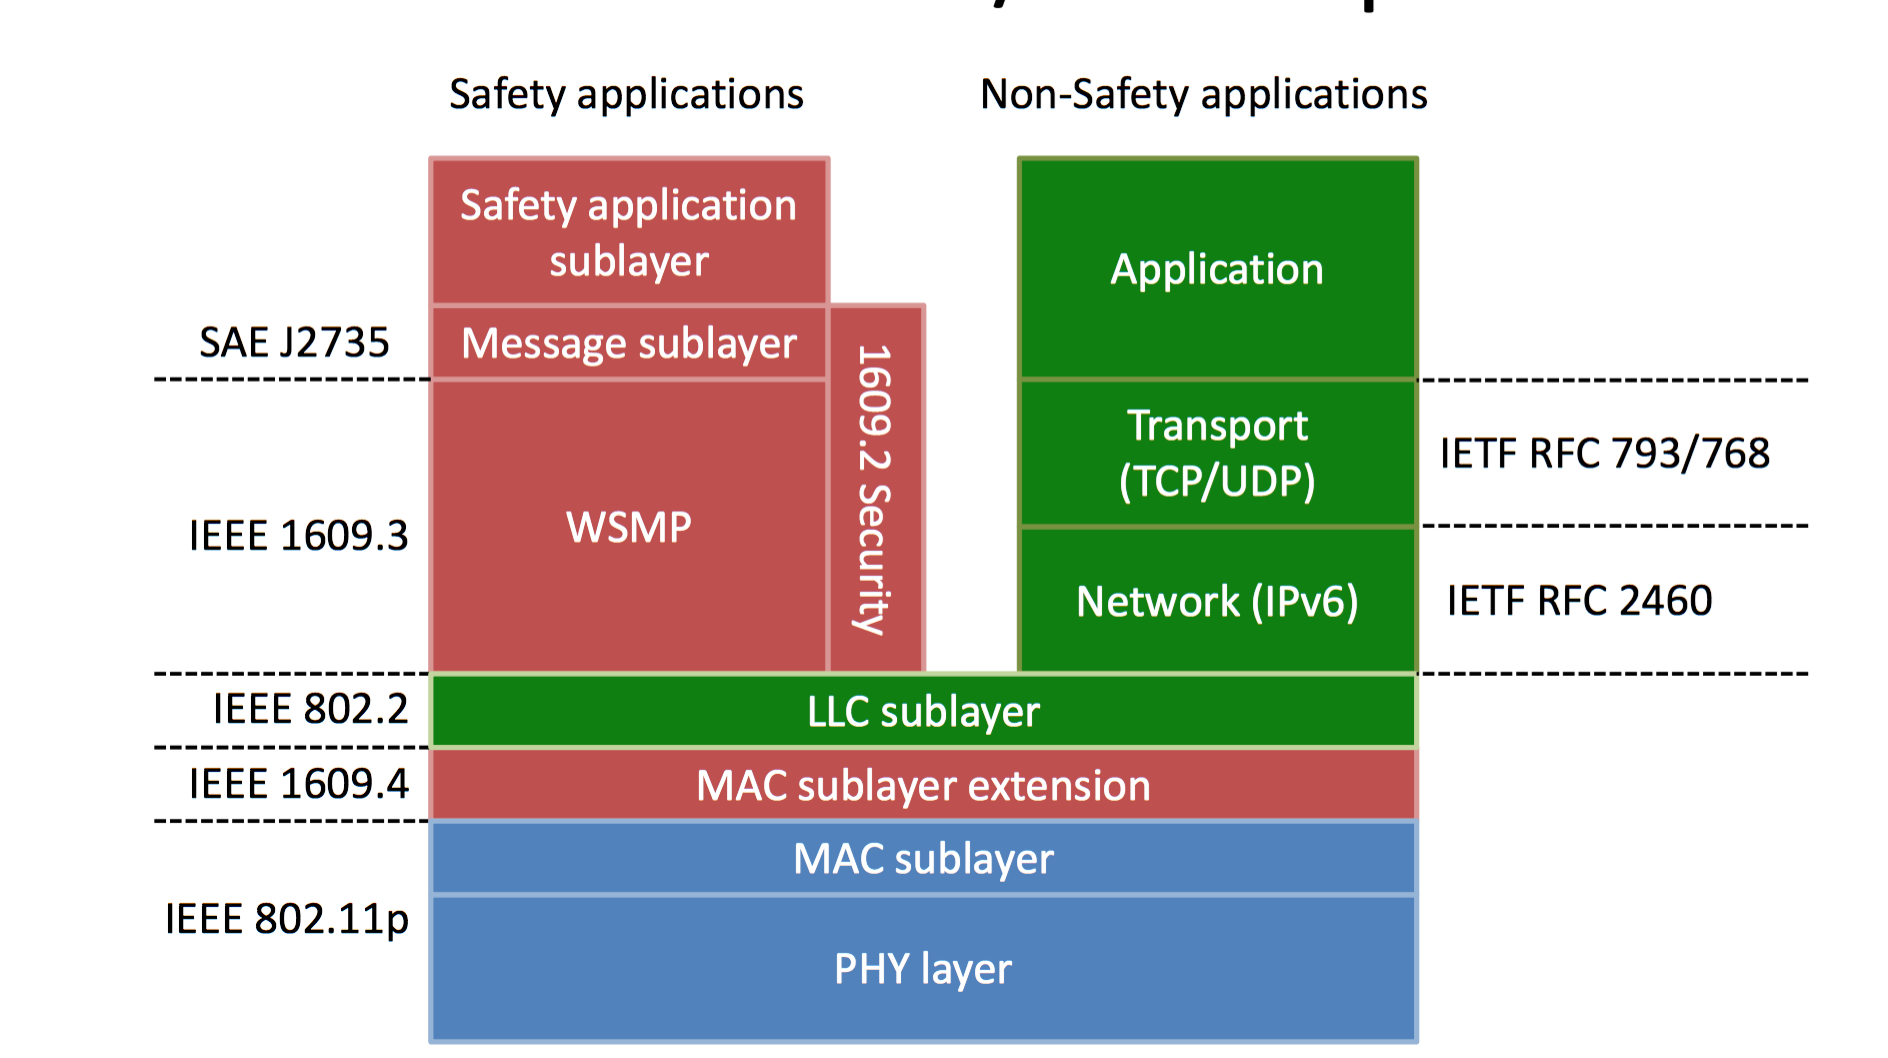
\includegraphics[width=0.7\columnwidth]{figures/WAVE_stack.png}
	\caption{A block diagrammatic illustration of the proposed technical approach.}
	\label{fig-project-block}
\end{figure}

The physical layer of VANET is derived from IEEE 802.11a with 3 different channel width options: 5MHz, 10MHz and 20MHz, among which 10MHz is recommended. Same with 802.11a, 802.11p is using Orthogonal Frequency Division Multiplexing (OFDM) including 52 carriers, 48 data carriers and 4 pilots, and 8 us symbol interval. The physical channel supports BPSK, SPSK,16QAM and 64QAM. 

\begin{figure}[h!]
	\centering
	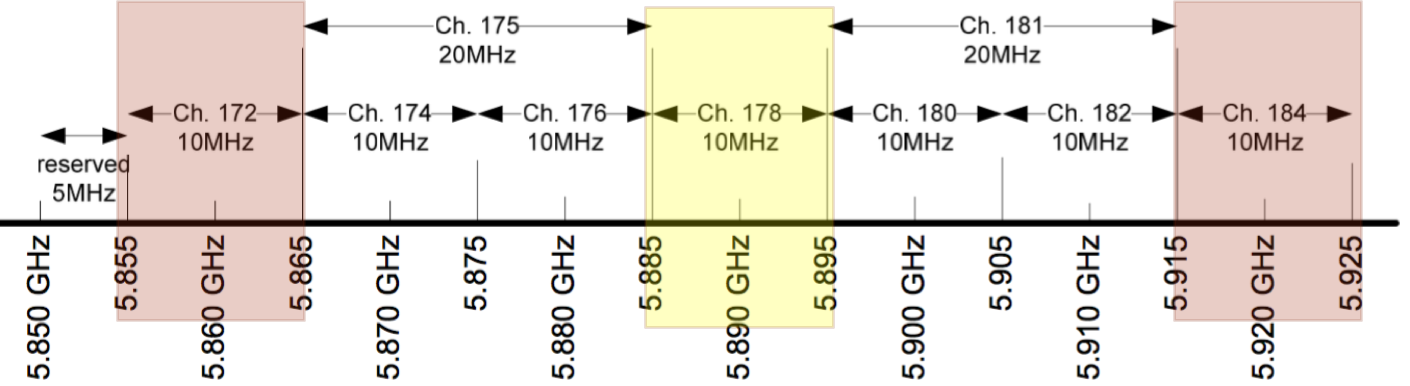
\includegraphics[width=0.7\columnwidth]{figures/DSRC_channel.png}
	\caption{A block diagrammatic illustration of the proposed technical approach.}
	\label{fig-project-block}
\end{figure}


For the purpose of supporting safety applications, Dedicated Short Range Communication (DSRC) is developed. 75MHz spectrum in 5.9GHz frequency band is allocated for DSRC application, which includes 1 control channel (CCH) and 6 service channels (SCH). The CCH is for transmitting high-priority short control messages and management data. Among the SCHs, FCC defines Ch. 172 and Ch. 184 special for safety applications.  SCH 172 is for V2V Safety communications for accident avoidance and mitigation, and safety of life and property applications. SCH 184 is for high-power, longer distance communications to be used for public safety applications involving safety of life and property, including road intersection collision mitigation. 

In order to decrease the latency of communication under the high mobility environment, the MAC layer of VANET is also changed. Both IEEE 802.11p and IEEE 1609.4 define new characteristics of the MAC layer. In IEEE802.11, the wireless nodes could form a Service Set (SS), in which the nodes have the same Service ID (SSID) and share communication. The network with Access Point (AP) is called Basic Service Set (BSS) while a network with no AP, i.e., ad-hoc network, is named Independent BSS (IBSS). Several BSS could connect together to form Extended Service Set (ESS), all the BSS in one ESS is sharing the same Extended SSID (ESSID). The problem is forming a SS before the communication happened may take a lot of time, which is not suitable for fast changing VANET. Therefore, IEEE 802.11p proposed out of the context of BSS (OCB). The OCB mode applies to multiple devices within the coverage area of a single radio link. In the OCB mode, the vehicle can send or receive data any time without forming or being a member of an SS. In addition, IEEE 802.11p removed authentication, association and data confidentiality mechanisms from MAC layer and moved them to an independent higher layer defined in IEEE 1609.2. On the other side, IEEE 802.11p still keep the BSS mode, this is mainly for infotainment applications via V2I communication. 

For medium access mechanism, traditional IEEE 802.11 is using Carrier Sense Multiple Access (CSMA)/Collision Avoidance (CA). IEEE 802.11p keeps CSMA, but not only that, it proposes Hybrid Coordination Function (HCF), which ensures Quality of Service (QoS) via Enhance Defense Cooperation Agreement (EDCA) defined in IEEE 802.11e. Data from different services has different priorities depend on the importance as shown in the table. 

\begin{figure}[h!]
	\centering
	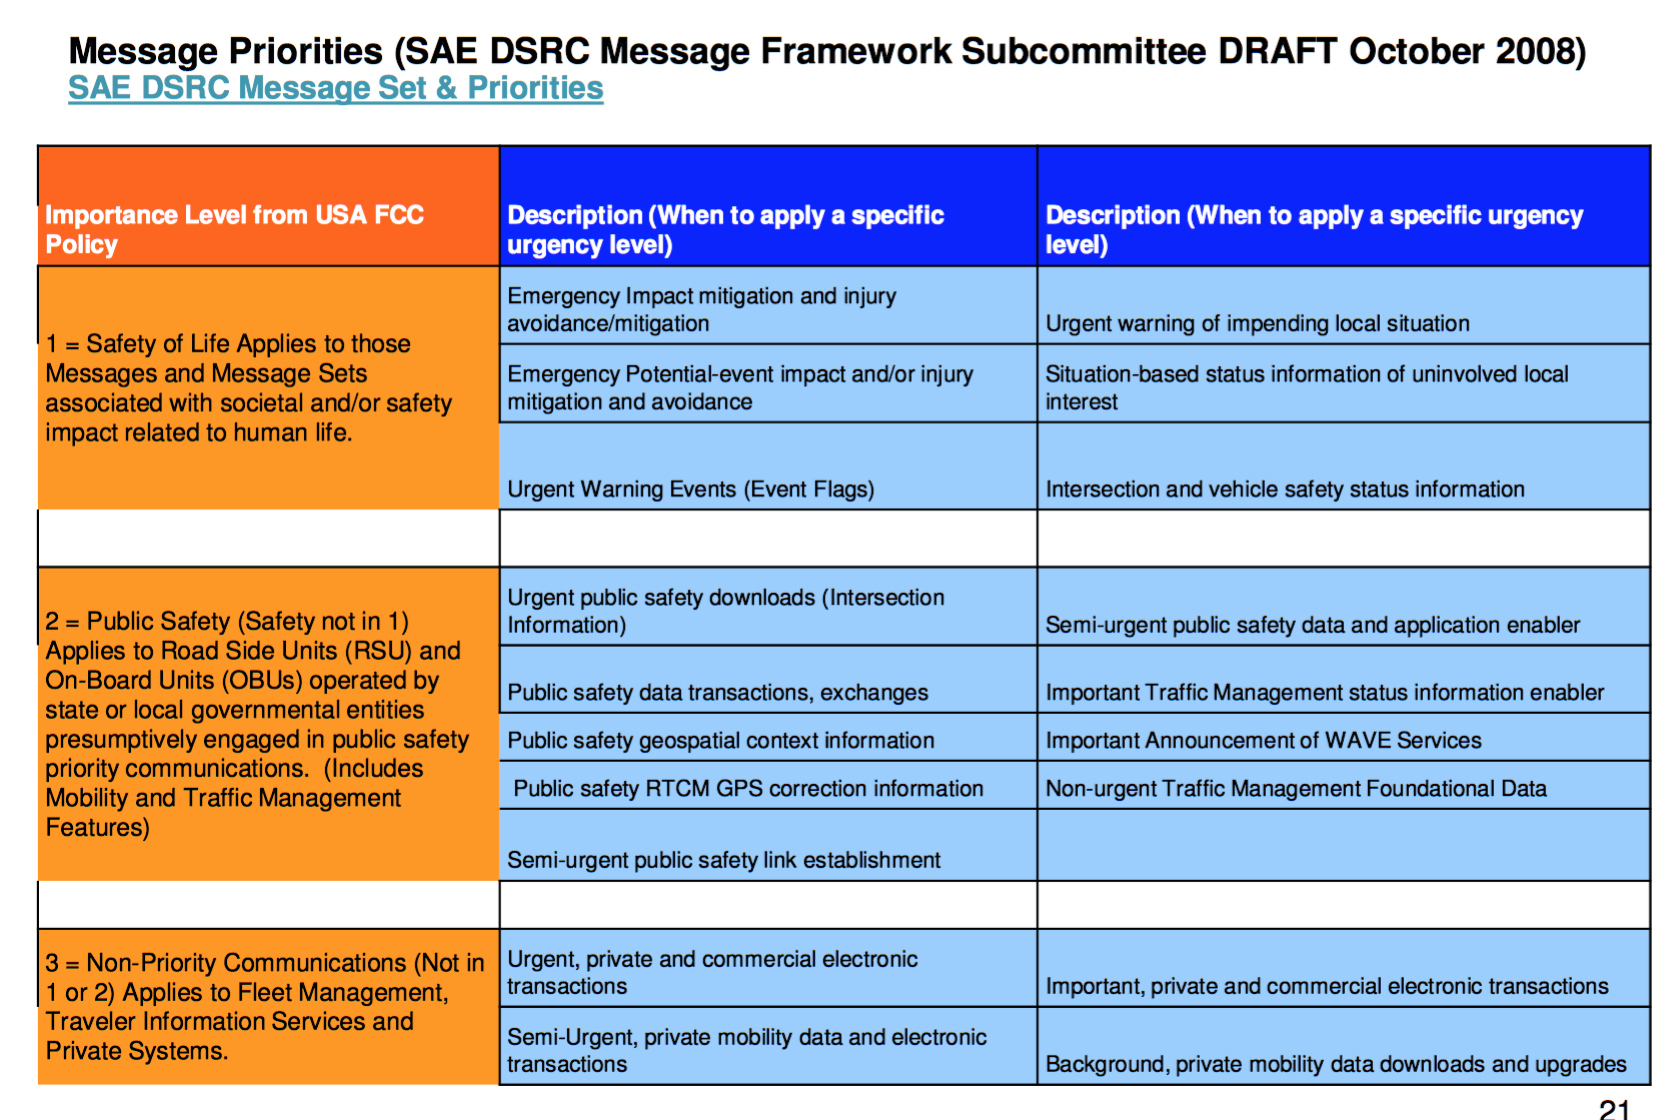
\includegraphics[width=0.7\columnwidth]{figures/msg_priority.png}
	\caption{A block diagrammatic illustration of the proposed technical approach.}
	\label{fig-project-block}
\end{figure}



In addition to the IEEE 802.11p, IEEE 1609.4 defines multi-channel behaviors in MAC layer of VANET. As the PHY layer of VANET has 7 channels, IEEE 1609.4 depicts the channel switching mechanism among the CCH and SCHs. 

IEEE 1609.3 defines two types of messages in VANET, Wave Short Message Protocol (WSMP) and IPv6 stack. IPv6 is usually for infotainment applications while the safety applications are transmitted via WAVE Short Messages (WSM). 

SAE standards are made for the safety messages. SAE J2735 defines 15 types of safety messages such as Basic Safety Messages (BSM), Signal Phase Time (SPT) and MAP message. Specially, BSM is broadcast periodically in 10Hz announcing state information such as position, speed, acceleration and heading direction etc. 

In addition, SAE J2945 specifies the minimum communication performance requirements of the SAE J2735 DSRC message sets and associated data frames and data elements. In order to ensure interoperability between vehicles, SAE J2945 further defines BSMs sending rate, transmit power control, and adaptive message rate control etc. 


----


Two current trends promise to revolutionize the safety, reliability, and energy-efficiency of 
future automotive transportation \cite{Barbaresso2014}: (i) wireless connectivity of vehicles 
to each other 
(Vehicle-to-Vehicle, or V2V), to smart infrastructure (Vehicle-to-Infrastructure, or V2I), 
and to other mobile devices, and (ii) autonomy, 
ranging from driver assistance (L1 systems), to full self-driving autonomy (L4 systems). 
Connected autonomous vehicles (CAVs) are cyber-physical systems (CPS) with increasingly 
complex software algorithms in control of a physical vehicle moving in uncertain real-world 
environments.\vspace{\parskip}


\textbf{The goal of this project is to investigate \textit{bidirectional} 
	interactions between the technologies of autonomy and of wireless connectivity in CPS. Using 
	CAVs as a case study in CPS, we propose to investigate how estimation and control algorithms 
	affect -- and are affected by -- software-defined radio communications in spectrum-scarce, 
	data-rich environments.}\vspace{\parskip} \markup{Copied from previous CPS proposal, should be changed}